\paragraph{Aim}
Considering that the maximal margin hyperplane is extremely sensitive
to a change in a single observation, it may have overfit the training
data.\\
In this case we might be willing to consider a classifier based on a
hyperplane that does not perfectly separate the 2 classes therewith to
get 
\begin{itemize}
	\item \tB{Greater robustness} to individual observation
	\item \tB{Better classification} of most of the training observations
\end{itemize}
And the \emph{Support Vector Classifier} does exactly this.

\paragraph{Details}
The support vector classifier classifies a test observation depending
on which side of the hyperplane it lies.
\begin{figure}[H]
	\begin{center}
		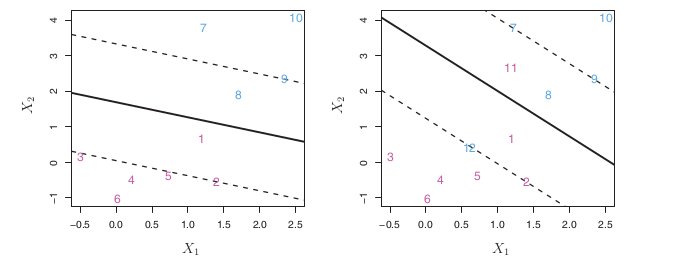
\includegraphics[width=\textwidth]{./chap/1chap/8sec/images/2supportVectorClassifier.png}
	\end{center}
	\caption{Left:Purple observations: 3, 4, 5 and 6 are on the 
	correct side, 2 is on the margin and 1 is on the wrong side.\\
	Blue observations: 7 and 10 are on the correct side, 9 on the
	margin and 8 on the wrong side\\
	Right: same as left panel with two additional points, 11 and 12
	which are on the wrong side}
	\label{fig:8.1 supportVectorClassifier}
\end{figure}

It is the solution to the optimization problem
\begin{center}
\enc{$
\max\limits_{\prtH{\beta}{i}{0}{p}\prtH{\epsilon}{i}{1}{n},M}~M~
\text{ subject to }
\begin{cases}
	\su{{j=1}}{p}\beta_{j}^{2}=1\\
	y_{i}\left( \beta_{0}+\su{{j=1}}{p}\beta_{j}x_{ij} \right) >
	M(1-\epsilon_{i})\\
	\epsilon_{i}\geq 0, \su{{i=1}}{n}\epsilon_{i}\leq C
\end{cases}$}
\end{center}
where $C$ is a nonnegative tuning parameter, $M$ is the width of the 
margin.\\
$\prth{\epsilon}{i}{n}$ are \emph{slack variables} that allow 
individual observations to be on the wrong side of the margin or the
hyperplane.
We have:
$$
\begin{cases}
	\tB{\epsilon_{i}=0}\Rightarrow i^{th}\text{ observation is on the
	\sB{correct side of the margin}}\\
	\tB{\epsilon_{i}>0}\Rightarrow i^{th}\text{ observation is on the
	\sB{wrong side of the margin}}\\
	\tB{\epsilon_{i}>1}\Rightarrow i^{th}\text{ observation is on the
	\sB{wrong side of the hyperplane}}\\
\end{cases}
$$
$C$ determines the number and severity of the violations to the margin
that we will tolerate.\\

In practice $C$ is treated as a tuning parameter that is generally 
chosen via cross-validation.\\

It turns out an observation that only observations that lies strictly
on the correct side of the margin does not affect the support vector
classifier.
